\documentclass[twoside]{book}

% Packages required by doxygen
\usepackage{fixltx2e}
\usepackage{calc}
\usepackage{doxygen}
\usepackage[export]{adjustbox} % also loads graphicx
\usepackage{graphicx}
\usepackage[utf8]{inputenc}
\usepackage{makeidx}
\usepackage{multicol}
\usepackage{multirow}
\PassOptionsToPackage{warn}{textcomp}
\usepackage{textcomp}
\usepackage[nointegrals]{wasysym}
\usepackage[table]{xcolor}

% NLS support packages
\usepackage[T2A]{fontenc}
\usepackage[russian]{babel}

% Font selection
\usepackage[T1]{fontenc}
\usepackage[scaled=.90]{helvet}
\usepackage{courier}
\usepackage{amssymb}
\usepackage{sectsty}
\renewcommand{\familydefault}{\sfdefault}
\allsectionsfont{%
  \fontseries{bc}\selectfont%
  \color{darkgray}%
}
\renewcommand{\DoxyLabelFont}{%
  \fontseries{bc}\selectfont%
  \color{darkgray}%
}
\newcommand{\+}{\discretionary{\mbox{\scriptsize$\hookleftarrow$}}{}{}}

% Page & text layout
\usepackage{geometry}
\geometry{%
  a4paper,%
  top=2.5cm,%
  bottom=2.5cm,%
  left=2.5cm,%
  right=2.5cm%
}
\tolerance=750
\hfuzz=15pt
\hbadness=750
\setlength{\emergencystretch}{15pt}
\setlength{\parindent}{0cm}
\setlength{\parskip}{3ex plus 2ex minus 2ex}
\makeatletter
\renewcommand{\paragraph}{%
  \@startsection{paragraph}{4}{0ex}{-1.0ex}{1.0ex}{%
    \normalfont\normalsize\bfseries\SS@parafont%
  }%
}
\renewcommand{\subparagraph}{%
  \@startsection{subparagraph}{5}{0ex}{-1.0ex}{1.0ex}{%
    \normalfont\normalsize\bfseries\SS@subparafont%
  }%
}
\makeatother

% Headers & footers
\usepackage{fancyhdr}
\pagestyle{fancyplain}
\fancyhead[LE]{\fancyplain{}{\bfseries\thepage}}
\fancyhead[CE]{\fancyplain{}{}}
\fancyhead[RE]{\fancyplain{}{\bfseries\leftmark}}
\fancyhead[LO]{\fancyplain{}{\bfseries\rightmark}}
\fancyhead[CO]{\fancyplain{}{}}
\fancyhead[RO]{\fancyplain{}{\bfseries\thepage}}
\fancyfoot[LE]{\fancyplain{}{}}
\fancyfoot[CE]{\fancyplain{}{}}
\fancyfoot[RE]{\fancyplain{}{\bfseries\scriptsize Создано системой Doxygen }}
\fancyfoot[LO]{\fancyplain{}{\bfseries\scriptsize Создано системой Doxygen }}
\fancyfoot[CO]{\fancyplain{}{}}
\fancyfoot[RO]{\fancyplain{}{}}
\renewcommand{\footrulewidth}{0.4pt}
\renewcommand{\chaptermark}[1]{%
  \markboth{#1}{}%
}
\renewcommand{\sectionmark}[1]{%
  \markright{\thesection\ #1}%
}

% Indices & bibliography
\usepackage{natbib}
\usepackage[titles]{tocloft}
\setcounter{tocdepth}{3}
\setcounter{secnumdepth}{5}
\makeindex

% Hyperlinks (required, but should be loaded last)
\usepackage{ifpdf}
\ifpdf
  \usepackage[pdftex,pagebackref=true]{hyperref}
\else
  \usepackage[ps2pdf,pagebackref=true]{hyperref}
\fi
\hypersetup{%
  colorlinks=true,%
  linkcolor=blue,%
  citecolor=blue,%
  unicode%
}

% Custom commands
\newcommand{\clearemptydoublepage}{%
  \newpage{\pagestyle{empty}\cleardoublepage}%
}

\usepackage{caption}
\captionsetup{labelsep=space,justification=centering,font={bf},singlelinecheck=off,skip=4pt,position=top}

%===== C O N T E N T S =====

\begin{document}

% Titlepage & ToC
\hypersetup{pageanchor=false,
             bookmarksnumbered=true,
             pdfencoding=unicode
            }
\pagenumbering{alph}
\begin{titlepage}
\vspace*{7cm}
\begin{center}%
{\Large СТЕГАНОГРАФИЧЕСКАЯ ПРОГРАММА, ИСПОЛЬЗУЮЩАЯ МЕТОД L\+SB ДЛЯ ИЗОБРАЖЕНИЙ В ФОРМАТЕ B\+MP }\\
\vspace*{1cm}
{\large Создано системой Doxygen 1.8.13}\\
\end{center}
\end{titlepage}
\clearemptydoublepage
\pagenumbering{roman}
\tableofcontents
\clearemptydoublepage
\pagenumbering{arabic}
\hypersetup{pageanchor=true}

%--- Begin generated contents ---
\chapter{Иерархический список классов}
\section{Иерархия классов}
Иерархия классов.\begin{DoxyCompactList}
\item \contentsline{section}{Bmp\+File}{\pageref{classBmpFile}}{}
\item invalid\+\_\+argument\begin{DoxyCompactList}
\item \contentsline{section}{cipher\+\_\+error}{\pageref{classcipher__error}}{}
\end{DoxyCompactList}
\end{DoxyCompactList}

\chapter{Алфавитный указатель классов}
\section{Классы}
Классы с их кратким описанием.\begin{DoxyCompactList}
\item\contentsline{section}{\hyperlink{classBmpFile}{Bmp\+File} }{\pageref{classBmpFile}}{}
\item\contentsline{section}{\hyperlink{classcipher__error}{cipher\+\_\+error} }{\pageref{classcipher__error}}{}
\end{DoxyCompactList}

\chapter{Список файлов}
\section{Файлы}
Полный список документированных файлов.\begin{DoxyCompactList}
\item\contentsline{section}{\hyperlink{bmpFile_8h}{bmp\+File.\+h} \\*Заголовочный файл для модуля Стеганографической программы методом L\+SB для изображений в формате B\+MP }{\pageref{bmpFile_8h}}{}
\item\contentsline{section}{{\bfseries header.\+h} }{\pageref{header_8h}}{}
\end{DoxyCompactList}

\chapter{Классы}
\hypertarget{classBmpFile}{}\section{Класс Bmp\+File}
\label{classBmpFile}\index{Bmp\+File@{Bmp\+File}}
\subsection*{Открытые члены}
\begin{DoxyCompactItemize}
\item 
\hyperlink{classBmpFile_aed9f5a62b69ee09e62f75ff70317e027}{Bmp\+File} (char $\ast$filename)
\begin{DoxyCompactList}\small\item\em конструктор для считывания файла \end{DoxyCompactList}\item 
int \hyperlink{classBmpFile_a4b19c02adb6237073491bd44e389d9f2}{is\+File\+Exist} (char $\ast$filename)
\begin{DoxyCompactList}\small\item\em открытие файла с изображением. \end{DoxyCompactList}\item 
int \hyperlink{classBmpFile_a917e862e4813dbef1a4e94fa67a83832}{get\+Dimension} (char $\ast$filename, long $\ast$width, long $\ast$height)
\begin{DoxyCompactList}\small\item\em получение высоты и ширины изображения. \end{DoxyCompactList}\item 
int \hyperlink{classBmpFile_aea6e2670a066a2967837c54323d7eaf0}{read\+Header} (char $\ast$filename)
\begin{DoxyCompactList}\small\item\em чтение загаловка файла с изображением. \end{DoxyCompactList}\item 
int \hyperlink{classBmpFile_a0ba2aa19f5b7d478a266bd0a162840b7}{hide} (char $\ast$bmpfile, char $\ast$txtfile, char $\ast$output)
\begin{DoxyCompactList}\small\item\em сокрытие информации. \end{DoxyCompactList}\item 
int \hyperlink{classBmpFile_adcc78879312808ffbe64dfadff699450}{unhide} (char $\ast$bmpfile, char $\ast$txtfile)
\begin{DoxyCompactList}\small\item\em извлечение информации. \end{DoxyCompactList}\item 
int \hyperlink{classBmpFile_abfcc28bca4d0113ad37ce2e1f2547a21}{check\+Files\+For\+Hiding} (char $\ast$bmpfile, char $\ast$txtfile)
\begin{DoxyCompactList}\small\item\em Проверка файлов для сокрытия. \end{DoxyCompactList}\item 
int \hyperlink{classBmpFile_acd76df84283673fd0bfc32b8edb8239b}{print\+File\+Info} ()
\begin{DoxyCompactList}\small\item\em вывод информации о изображении \end{DoxyCompactList}\end{DoxyCompactItemize}
\subsection*{Открытые атрибуты}
\begin{DoxyCompactItemize}
\item 
int \hyperlink{classBmpFile_a74c74bb4fbe13d87e5380c5a51ce1bd1}{bmp\+Identifier}
\begin{DoxyCompactList}\small\item\em Стеганография \end{DoxyCompactList}\item 
\mbox{\Hypertarget{classBmpFile_a42dba4f718cb942205c3b0550e7e992f}\label{classBmpFile_a42dba4f718cb942205c3b0550e7e992f}} 
long {\bfseries bmp\+Filesize}
\item 
\mbox{\Hypertarget{classBmpFile_aea570822938beb63dd2804c5ff9ff3ab}\label{classBmpFile_aea570822938beb63dd2804c5ff9ff3ab}} 
unsigned short int {\bfseries bmpres1}
\item 
\mbox{\Hypertarget{classBmpFile_a73b58b3475074d19a83e6072f371392d}\label{classBmpFile_a73b58b3475074d19a83e6072f371392d}} 
unsigned short int {\bfseries bmpres2}
\item 
\mbox{\Hypertarget{classBmpFile_a7cfeb8d372eb1f236f134ff87b6600ad}\label{classBmpFile_a7cfeb8d372eb1f236f134ff87b6600ad}} 
long {\bfseries bmp\+Pixoff}
\item 
\mbox{\Hypertarget{classBmpFile_a8a91127964f183702055c14b329213be}\label{classBmpFile_a8a91127964f183702055c14b329213be}} 
long {\bfseries bmpi\+Size}
\item 
\mbox{\Hypertarget{classBmpFile_a0fd9f4b5be9b6aab6fa41ec8dcc643de}\label{classBmpFile_a0fd9f4b5be9b6aab6fa41ec8dcc643de}} 
long {\bfseries bmp\+Width}
\item 
\mbox{\Hypertarget{classBmpFile_a3049ef9d773c8f1b2fb2ad7edae40f4f}\label{classBmpFile_a3049ef9d773c8f1b2fb2ad7edae40f4f}} 
long {\bfseries bmp\+Height}
\item 
\mbox{\Hypertarget{classBmpFile_a06fffe85623bb795a26f88667cc47452}\label{classBmpFile_a06fffe85623bb795a26f88667cc47452}} 
unsigned short int {\bfseries bmp\+Planes}
\item 
\mbox{\Hypertarget{classBmpFile_a98e8f1725115e6b41577ae6dd65c82a1}\label{classBmpFile_a98e8f1725115e6b41577ae6dd65c82a1}} 
unsigned short int {\bfseries bmp\+Bits\+Pixel}
\item 
\mbox{\Hypertarget{classBmpFile_a00e26fc5aa496f1d3e244d934a5d3bc6}\label{classBmpFile_a00e26fc5aa496f1d3e244d934a5d3bc6}} 
long {\bfseries bmp\+Compression}
\item 
\mbox{\Hypertarget{classBmpFile_aa1b582e76207d2906a28e8ba29687f4a}\label{classBmpFile_aa1b582e76207d2906a28e8ba29687f4a}} 
long {\bfseries bmp\+Image\+Size}
\item 
\mbox{\Hypertarget{classBmpFile_aefcbdfc073a8dbdb2742f8d03ae8f7de}\label{classBmpFile_aefcbdfc073a8dbdb2742f8d03ae8f7de}} 
long {\bfseries bmp\+Xscale}
\item 
\mbox{\Hypertarget{classBmpFile_a6a57a0ab219996baf7a4df37b0c2f857}\label{classBmpFile_a6a57a0ab219996baf7a4df37b0c2f857}} 
long {\bfseries bmp\+Y\+Scale}
\item 
\mbox{\Hypertarget{classBmpFile_a460c34ddeb210b7785c62896ce2d06ea}\label{classBmpFile_a460c34ddeb210b7785c62896ce2d06ea}} 
long {\bfseries bmp\+Color}
\item 
\mbox{\Hypertarget{classBmpFile_afc9ef75ec2ce08ec94feb37eaa4a19f1}\label{classBmpFile_afc9ef75ec2ce08ec94feb37eaa4a19f1}} 
long {\bfseries bmp\+Imp\+Col}
\item 
\mbox{\Hypertarget{classBmpFile_a6b16f42aebee776362cc4079951e3ca8}\label{classBmpFile_a6b16f42aebee776362cc4079951e3ca8}} 
long {\bfseries bmp\+Total\+Stuffablechar}
\end{DoxyCompactItemize}


\subsection{Конструктор(ы)}
\mbox{\Hypertarget{classBmpFile_aed9f5a62b69ee09e62f75ff70317e027}\label{classBmpFile_aed9f5a62b69ee09e62f75ff70317e027}} 
\index{Bmp\+File@{Bmp\+File}!Bmp\+File@{Bmp\+File}}
\index{Bmp\+File@{Bmp\+File}!Bmp\+File@{Bmp\+File}}
\subsubsection{\texorpdfstring{Bmp\+File()}{BmpFile()}}
{\footnotesize\ttfamily Bmp\+File\+::\+Bmp\+File (\begin{DoxyParamCaption}\item[{char $\ast$}]{filename }\end{DoxyParamCaption})}



конструктор для считывания файла 


\begin{DoxyParams}[1]{Аргументы}
\mbox{\tt in}  & {\em filename} & файл. Формат B\+MP \\
\hline
\end{DoxyParams}

\begin{DoxyExceptions}{Исключения}
{\em \hyperlink{classcipher__error}{cipher\+\_\+error},если} & неверный формат изображения. \\
\hline
\end{DoxyExceptions}


\subsection{Методы}
\mbox{\Hypertarget{classBmpFile_abfcc28bca4d0113ad37ce2e1f2547a21}\label{classBmpFile_abfcc28bca4d0113ad37ce2e1f2547a21}} 
\index{Bmp\+File@{Bmp\+File}!check\+Files\+For\+Hiding@{check\+Files\+For\+Hiding}}
\index{check\+Files\+For\+Hiding@{check\+Files\+For\+Hiding}!Bmp\+File@{Bmp\+File}}
\subsubsection{\texorpdfstring{check\+Files\+For\+Hiding()}{checkFilesForHiding()}}
{\footnotesize\ttfamily int Bmp\+File\+::check\+Files\+For\+Hiding (\begin{DoxyParamCaption}\item[{char $\ast$}]{bmpfile,  }\item[{char $\ast$}]{txtfile }\end{DoxyParamCaption})}



Проверка файлов для сокрытия. 


\begin{DoxyParams}[1]{Аргументы}
\mbox{\tt in}  & {\em bmpfile} & файл. Формат B\+MP \\
\hline
\mbox{\tt in}  & {\em txtfile} & файл. \\
\hline
\end{DoxyParams}
\begin{DoxyReturn}{Возвращает}
целочисленное значение. 
\end{DoxyReturn}

\begin{DoxyExceptions}{Исключения}
{\em \hyperlink{classcipher__error}{cipher\+\_\+error},если} & неверный формат изображения. если не удалось открыть какой-\/то из файлов сообщение длинне возможного сокрытия. \\
\hline
\end{DoxyExceptions}
\mbox{\Hypertarget{classBmpFile_a917e862e4813dbef1a4e94fa67a83832}\label{classBmpFile_a917e862e4813dbef1a4e94fa67a83832}} 
\index{Bmp\+File@{Bmp\+File}!get\+Dimension@{get\+Dimension}}
\index{get\+Dimension@{get\+Dimension}!Bmp\+File@{Bmp\+File}}
\subsubsection{\texorpdfstring{get\+Dimension()}{getDimension()}}
{\footnotesize\ttfamily int Bmp\+File\+::get\+Dimension (\begin{DoxyParamCaption}\item[{char $\ast$}]{filename,  }\item[{long $\ast$}]{width,  }\item[{long $\ast$}]{height }\end{DoxyParamCaption})}



получение высоты и ширины изображения. 


\begin{DoxyParams}[1]{Аргументы}
\mbox{\tt in}  & {\em filename} & файл. Формат B\+MP \\
\hline
\mbox{\tt in}  & {\em width} & ширина. \\
\hline
\mbox{\tt in}  & {\em height} & высота. \\
\hline
\end{DoxyParams}
\begin{DoxyReturn}{Возвращает}
целочисленное значение. 
\end{DoxyReturn}

\begin{DoxyExceptions}{Исключения}
{\em \hyperlink{classcipher__error}{cipher\+\_\+error},если} & неверный формат изображения. \\
\hline
\end{DoxyExceptions}
\mbox{\Hypertarget{classBmpFile_a0ba2aa19f5b7d478a266bd0a162840b7}\label{classBmpFile_a0ba2aa19f5b7d478a266bd0a162840b7}} 
\index{Bmp\+File@{Bmp\+File}!hide@{hide}}
\index{hide@{hide}!Bmp\+File@{Bmp\+File}}
\subsubsection{\texorpdfstring{hide()}{hide()}}
{\footnotesize\ttfamily int Bmp\+File\+::hide (\begin{DoxyParamCaption}\item[{char $\ast$}]{bmpfile,  }\item[{char $\ast$}]{txtfile,  }\item[{char $\ast$}]{output }\end{DoxyParamCaption})}



сокрытие информации. 


\begin{DoxyParams}[1]{Аргументы}
\mbox{\tt in}  & {\em bmpfile} & файл. Формат B\+MP \\
\hline
\mbox{\tt in}  & {\em txtfile} & файл. \\
\hline
\mbox{\tt in}  & {\em output} & файл. Формат B\+MP \\
\hline
\end{DoxyParams}
\begin{DoxyReturn}{Возвращает}
целочисленное значение. 
\end{DoxyReturn}

\begin{DoxyExceptions}{Исключения}
{\em \hyperlink{classcipher__error}{cipher\+\_\+error},если} & неверный формат изображения. если не удалось открыть какой-\/то из файлов сообщение длинне возможного сокрытия. \\
\hline
\end{DoxyExceptions}
\mbox{\Hypertarget{classBmpFile_a4b19c02adb6237073491bd44e389d9f2}\label{classBmpFile_a4b19c02adb6237073491bd44e389d9f2}} 
\index{Bmp\+File@{Bmp\+File}!is\+File\+Exist@{is\+File\+Exist}}
\index{is\+File\+Exist@{is\+File\+Exist}!Bmp\+File@{Bmp\+File}}
\subsubsection{\texorpdfstring{is\+File\+Exist()}{isFileExist()}}
{\footnotesize\ttfamily int Bmp\+File\+::is\+File\+Exist (\begin{DoxyParamCaption}\item[{char $\ast$}]{filename }\end{DoxyParamCaption})}



открытие файла с изображением. 


\begin{DoxyParams}[1]{Аргументы}
\mbox{\tt in}  & {\em filename} & файл. Формат B\+MP \\
\hline
\end{DoxyParams}
\begin{DoxyReturn}{Возвращает}
целочисленное значение. 
\end{DoxyReturn}

\begin{DoxyExceptions}{Исключения}
{\em \hyperlink{classcipher__error}{cipher\+\_\+error},если} & открыть не получилось. \\
\hline
\end{DoxyExceptions}
\mbox{\Hypertarget{classBmpFile_acd76df84283673fd0bfc32b8edb8239b}\label{classBmpFile_acd76df84283673fd0bfc32b8edb8239b}} 
\index{Bmp\+File@{Bmp\+File}!print\+File\+Info@{print\+File\+Info}}
\index{print\+File\+Info@{print\+File\+Info}!Bmp\+File@{Bmp\+File}}
\subsubsection{\texorpdfstring{print\+File\+Info()}{printFileInfo()}}
{\footnotesize\ttfamily int Bmp\+File\+::print\+File\+Info (\begin{DoxyParamCaption}{ }\end{DoxyParamCaption})}



вывод информации о изображении 

\begin{DoxyReturn}{Возвращает}
целочисленное значение. 
\end{DoxyReturn}
\mbox{\Hypertarget{classBmpFile_aea6e2670a066a2967837c54323d7eaf0}\label{classBmpFile_aea6e2670a066a2967837c54323d7eaf0}} 
\index{Bmp\+File@{Bmp\+File}!read\+Header@{read\+Header}}
\index{read\+Header@{read\+Header}!Bmp\+File@{Bmp\+File}}
\subsubsection{\texorpdfstring{read\+Header()}{readHeader()}}
{\footnotesize\ttfamily int Bmp\+File\+::read\+Header (\begin{DoxyParamCaption}\item[{char $\ast$}]{filename }\end{DoxyParamCaption})}



чтение загаловка файла с изображением. 


\begin{DoxyParams}[1]{Аргументы}
\mbox{\tt in}  & {\em filename} & файл. Формат B\+MP \\
\hline
\end{DoxyParams}
\begin{DoxyReturn}{Возвращает}
целочисленное значение. 
\end{DoxyReturn}

\begin{DoxyExceptions}{Исключения}
{\em \hyperlink{classcipher__error}{cipher\+\_\+error},если} & неверный формат изображения. \\
\hline
\end{DoxyExceptions}
\mbox{\Hypertarget{classBmpFile_adcc78879312808ffbe64dfadff699450}\label{classBmpFile_adcc78879312808ffbe64dfadff699450}} 
\index{Bmp\+File@{Bmp\+File}!unhide@{unhide}}
\index{unhide@{unhide}!Bmp\+File@{Bmp\+File}}
\subsubsection{\texorpdfstring{unhide()}{unhide()}}
{\footnotesize\ttfamily int Bmp\+File\+::unhide (\begin{DoxyParamCaption}\item[{char $\ast$}]{bmpfile,  }\item[{char $\ast$}]{txtfile }\end{DoxyParamCaption})}



извлечение информации. 


\begin{DoxyParams}[1]{Аргументы}
\mbox{\tt in}  & {\em bmpfile} & файл. Формат B\+MP \\
\hline
\mbox{\tt in}  & {\em txtfile} & файл. \\
\hline
\end{DoxyParams}
\begin{DoxyReturn}{Возвращает}
целочисленное значение. 
\end{DoxyReturn}

\begin{DoxyExceptions}{Исключения}
{\em \hyperlink{classcipher__error}{cipher\+\_\+error},если} & неверный формат изображения. если не удалось открыть какой-\/то из файлов \\
\hline
\end{DoxyExceptions}


\subsection{Данные класса}
\mbox{\Hypertarget{classBmpFile_a74c74bb4fbe13d87e5380c5a51ce1bd1}\label{classBmpFile_a74c74bb4fbe13d87e5380c5a51ce1bd1}} 
\index{Bmp\+File@{Bmp\+File}!bmp\+Identifier@{bmp\+Identifier}}
\index{bmp\+Identifier@{bmp\+Identifier}!Bmp\+File@{Bmp\+File}}
\subsubsection{\texorpdfstring{bmp\+Identifier}{bmpIdentifier}}
{\footnotesize\ttfamily int Bmp\+File\+::bmp\+Identifier}



Стеганография 

Контейнер устанавливается в конструкторе. Для записи и извлечения преднзначены соответственно методы hide, unhide. \begin{DoxyWarning}{Предупреждения}
Только для изображений формата B\+MP 
\end{DoxyWarning}


Объявления и описания членов классов находятся в файлах\+:\begin{DoxyCompactItemize}
\item 
\hyperlink{bmpFile_8h}{bmp\+File.\+h}\item 
bmp\+File.\+cpp\end{DoxyCompactItemize}

\hypertarget{classcipher__error}{}\section{Класс cipher\+\_\+error}
\label{classcipher__error}\index{cipher\+\_\+error@{cipher\+\_\+error}}


Граф наследования\+:cipher\+\_\+error\+:
\nopagebreak
\begin{figure}[H]
\begin{center}
\leavevmode
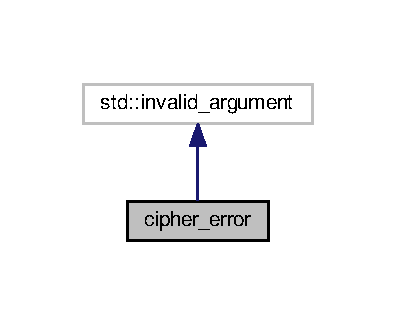
\includegraphics[width=190pt]{classcipher__error__inherit__graph}
\end{center}
\end{figure}


Граф связей класса cipher\+\_\+error\+:
\nopagebreak
\begin{figure}[H]
\begin{center}
\leavevmode
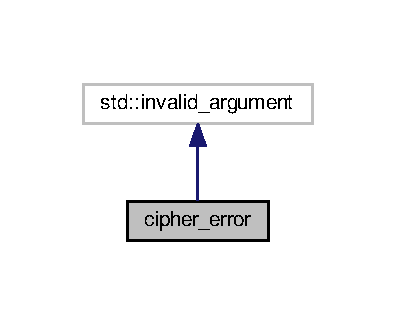
\includegraphics[width=190pt]{classcipher__error__coll__graph}
\end{center}
\end{figure}
\subsection*{Открытые члены}
\begin{DoxyCompactItemize}
\item 
\mbox{\Hypertarget{classcipher__error_aac662e216a84bfeb873303c7b88d029e}\label{classcipher__error_aac662e216a84bfeb873303c7b88d029e}} 
{\bfseries cipher\+\_\+error} (const std\+::string \&what\+\_\+arg)
\item 
\mbox{\Hypertarget{classcipher__error_a18cf27d9c2cd2538d3cb8f17e9a55f3e}\label{classcipher__error_a18cf27d9c2cd2538d3cb8f17e9a55f3e}} 
{\bfseries cipher\+\_\+error} (const char $\ast$what\+\_\+arg)
\end{DoxyCompactItemize}


Объявления и описания членов класса находятся в файле\+:\begin{DoxyCompactItemize}
\item 
\hyperlink{bmpFile_8h}{bmp\+File.\+h}\end{DoxyCompactItemize}

\chapter{Файлы}
\hypertarget{bmpFile_8h}{}\section{Файл bmp\+File.\+h}
\label{bmpFile_8h}\index{bmp\+File.\+h@{bmp\+File.\+h}}


Заголовочный файл для модуля Стеганографической программы методом L\+SB для изображений в формате B\+MP.  


\subsection*{Классы}
\begin{DoxyCompactItemize}
\item 
class \hyperlink{classBmpFile}{Bmp\+File}
\item 
class \hyperlink{classcipher__error}{cipher\+\_\+error}
\end{DoxyCompactItemize}


\subsection{Подробное описание}
Заголовочный файл для модуля Стеганографической программы методом L\+SB для изображений в формате B\+MP. 

\begin{DoxyAuthor}{Автор}
Колясов М.\+М. 
\end{DoxyAuthor}
\begin{DoxyVersion}{Версия}
1.\+0 
\end{DoxyVersion}
\begin{DoxyDate}{Дата}
13.\+06.\+2019 
\end{DoxyDate}
\begin{DoxyCopyright}{Авторство}
ИБСТ ПГУ 
\end{DoxyCopyright}
\begin{DoxyWarning}{Предупреждения}
Это учебный пример 
\end{DoxyWarning}

%--- End generated contents ---

% Index
\backmatter
\newpage
\phantomsection
\clearemptydoublepage
\addcontentsline{toc}{chapter}{Алфавитный указатель}
\printindex

\end{document}
